\clearpage
\subsection{Structure of web applications}
\label{sec:background-structure}

Web pages can be characterized by clients fetching web pages from servers and displaying the pages in web browsers. The basic building blocks for a web page are HyperText Markup Language (HTML) elements, which describe the structure and content of the page. The layout and style of web pages can be modified by using Cascading Style Sheets (CSS). The addition of JavaScript makes it possible for the browser to execute arbitrary code, greatly improving the options for interactive pages. 
Since its inception in the 80's, the web has evolved and matured. From static, read-only pages utilizing HTML to pages allowing users to write and participate in the web during the turn of the millennium, made possible in part by the adoption of JavaScript. The evolution continued to allow users to execute programs that we commonly refer to as web applications today \citep{jacksi_development_2019}. 


\subsubsection{Static web pages}
A traditional, static web page is stored in its entirety on the server and is served to users on request. 
Such pages typically require only HTML and CSS to function.
As the client side barely includes any logic, the focus is on the server, which stores and serves data and handles all business logic.
Navigation and interaction with the page is done using clickable links that direct the user to other pages.
Figure \ref{static} describes a user visiting a web page \textit{example.com}, clicking a link to visit \textit{example.com/apply} and finally submitting a form to \textit{example.com/apply}.
Keeping the content strictly separated in pages and serving the complete page as-is to clients provides a number of benefits \citep{camden_why_nodate}:

\begin{itemize}
    \item The amount of data transferred when visiting a site is low, as only the content that is immediately shown to the user has to be sent. This speeds up load times for the end user, reduces data usage and typically leads to a lower delay before content is visible in the browser.
    \item Static websites are typically easier to traverse programmatically than dynamic sites. This makes it easier for web crawlers to index the site, such as those used by search engines, making search engine optimization (SEO) trivial. Additionally, static sites are typically more accessible as they can be parsed more easily by screen readers and similar software \citep{okoye_accessibility_2014}.
    \item As the use of JavaScript allows websites to execute near arbitrary code in browsers, users can choose to disable JavaScript altogether. This will cause most dynamic sites to stop working, while static websites can function without using JavaScript. This removes the option for potential attackers to execute harmful code on the user's machine and often limits the tracking capabilities of websites. 
\end{itemize}

There are, however, reasons why strictly static sites are rare today, compared to the early days of the web when they were the standard \citep{nath_web_2014}:

\begin{itemize}
    \item Static websites are slow and clunky to use, as any interaction with the site requires the client to fetch a new page, or reload the current page from the server.
    \item Static websites only support client-initiated requests, making it impossible for the server to implement event-driven patterns, such as sending notifications to the client.
    \item Continually updating pages is not possible, as doing so would require server-initiated communication. The problem could be solved by the client periodically requesting the latest data, but this is not possible in strictly static sites as it requires JavaScript to implement.
\end{itemize}

\begin{figure}[b]
	\centering
	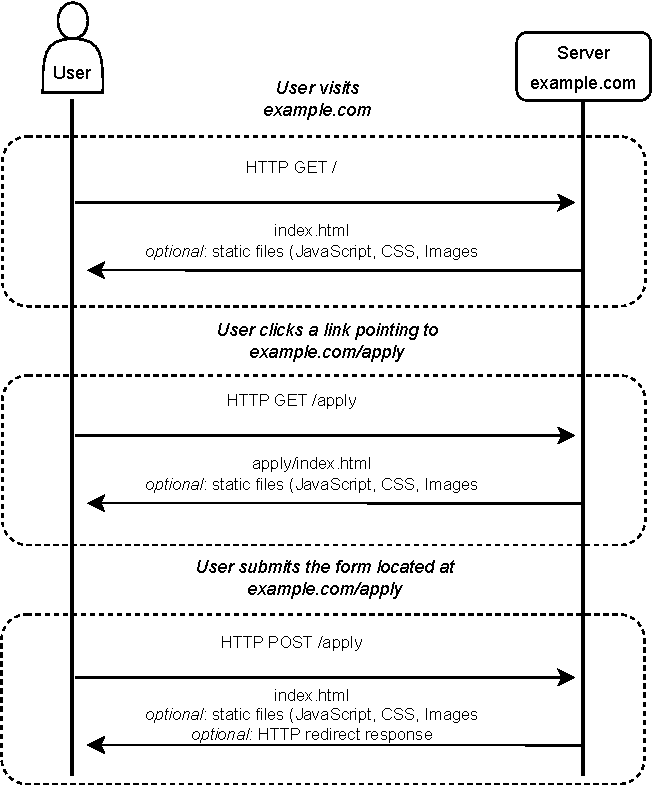
\includegraphics[height=120mm]{assets/http_request.drawio.pdf}
	\caption{Network traffic for a user interacting with a static web site.}
	\label{static}
\end{figure}

\subsubsection{Rich internet applications}

To allow for client-side scripting and alleviate some of the issues with strictly static sites, JavaScript was introduced in the mid 90's. While this allowed developers to create dynamic user interfaces, web apps as we know them today did not become popular until the introduction of third-party tools, such as Adobe Flash and Java in web apps. These technologies allowed for the development of rich internet applications (RIAs) that delegated some logic and data storage to the client, while using separate HTML pages for different pages \citep{fraternali_rich_2010}.
While these tools allowed for the creation of interactive web apps, end users had to install the tools separately if they wanted to utilize them. In addition to being a hassle for end users, these plugins introduced additional security vulnerabilities. At the time of writing, 1084 common vulnerabilities and exposures (CVEs) have been reported for Adobe Flash \citep{noauthor_adobe_nodate}.

Some way to create interactive web apps using only HTML, CSS and JavaScript was needed. The adoption of Asynchronous JavaScript and XML (Ajax) around 2005 saw web development move towards JavaScript-based applications that are common today. 
The asynchronous nature of Ajax allowed for completing network requests in the background without blocking user input and updating relevant parts of the interface when the request completed. 
JavaScript-based abstractions built on top of Ajax made development easier, such as jQuery \citep{openjsforg_jquery_nodate}, released in 2006, and the fetch() function \citep{noauthor_fetch_2023}, released in 2015. 

\subsubsection{Single-page applications}

Logic can further be delegated to the client, allowing for single-page applications (SPAs), that contain all the web pages for an application in one HTML page
\citep{fink_introducing_2014}. 
While the name might imply that SPAs only have one page, they can have any number of pages visible from the end users point of view, with the term \textit{single page} referring to the number of HTML pages.
In contrast to static web applications and RIAs, SPAs use client side logic instead of full HTTP requests to handle navigation and user input.
This often leads to improved responsiveness for users and makes dealing with client-side data and state easier, at the cost of a longer initial load time due to the larger size of the page.
The backend typically consists of an application programming interface (API), which is designed for machine communication with responses that might not be easily human-readable.
The backend and frontend often utilize JavaScript Object Notation (JSON) data to communicate.

Figure \ref{spa} shows the network traffic between a user and a web server for a simple SPA.
When comparing the traffic with the static page traffic in figure 2, the static page always returns a complete HTML page and redirects the user accordingly, while the SPA only fetches one HTML page on the initial page load.
The requests for the user navigating to \textit{/apply} and the user submitting a form can be identical for both the static page and the SPA.
The response from the backend is however different, with the static application returning a complete page and the SPA returning data in any suitable format, typically JSON.

\begin{figure}[b]
	\centering
	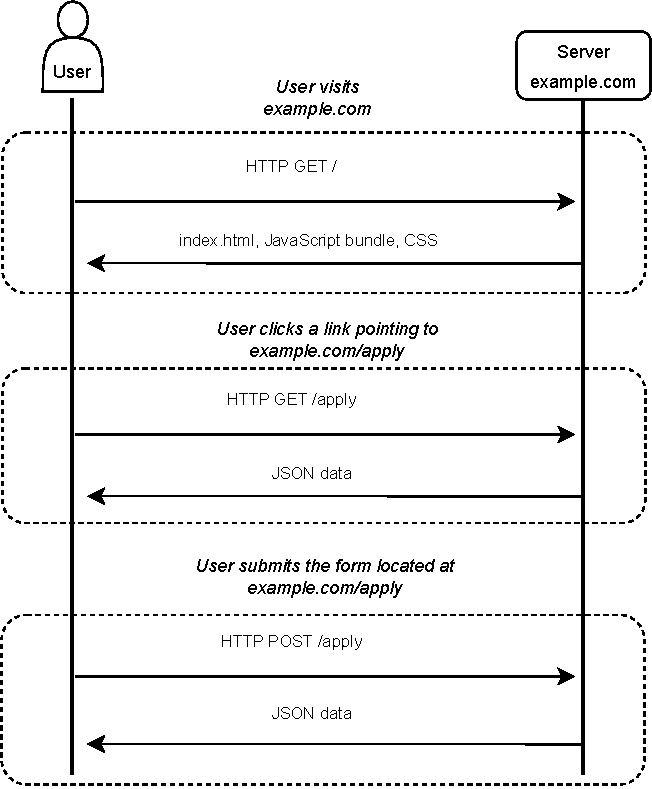
\includegraphics[height=120mm]{assets/spa_http_request.drawio.pdf}
	\caption{Network traffic for a user interacting with a Single Page Application.}
	\label{spa}
\end{figure}

While the network traffic of the SPA and static web page might seem very similar at first, there are many practical differences \citep{fink_introducing_2014}.
As SPAs implement navigation in the client, user navigation could be achieved without any network traffic, completely relying on the content of the first page load.
In practice some network traffic is often useful when navigating a SPA. 
Dynamic information can be fetched on navigation, periodically by the client or on-demand by the server, as data fetched on initial page load could easily become stale.
Pre-rendered HTML and static content such as images can also be fetched on navigation, lowering the size of the initial HTML page.
With SPAs, developers are given greater freedom in implementation, having the option to develop web applications very similarly to native applications, while not requiring end users to install anything on their machines.
While moving much of the logic to the client can make applications more responsive, moving logic from an opaque server to a transparent client application requires developers to pay attention to which parts they could move to the client.
In general, developers should assume that all data and application logic that is located in the client can be freely accessed and modified by potential attackers.

